It can be clearly seen that $\Delta$V budget is almost five times (CHECK) larger at low altitude at solar maximum when compared to the solar minimum. Overall the values for $\Delta$V at high altitudes, at solar minimum and time average look very favorable. 

\begin{figure}[h!]
\centering
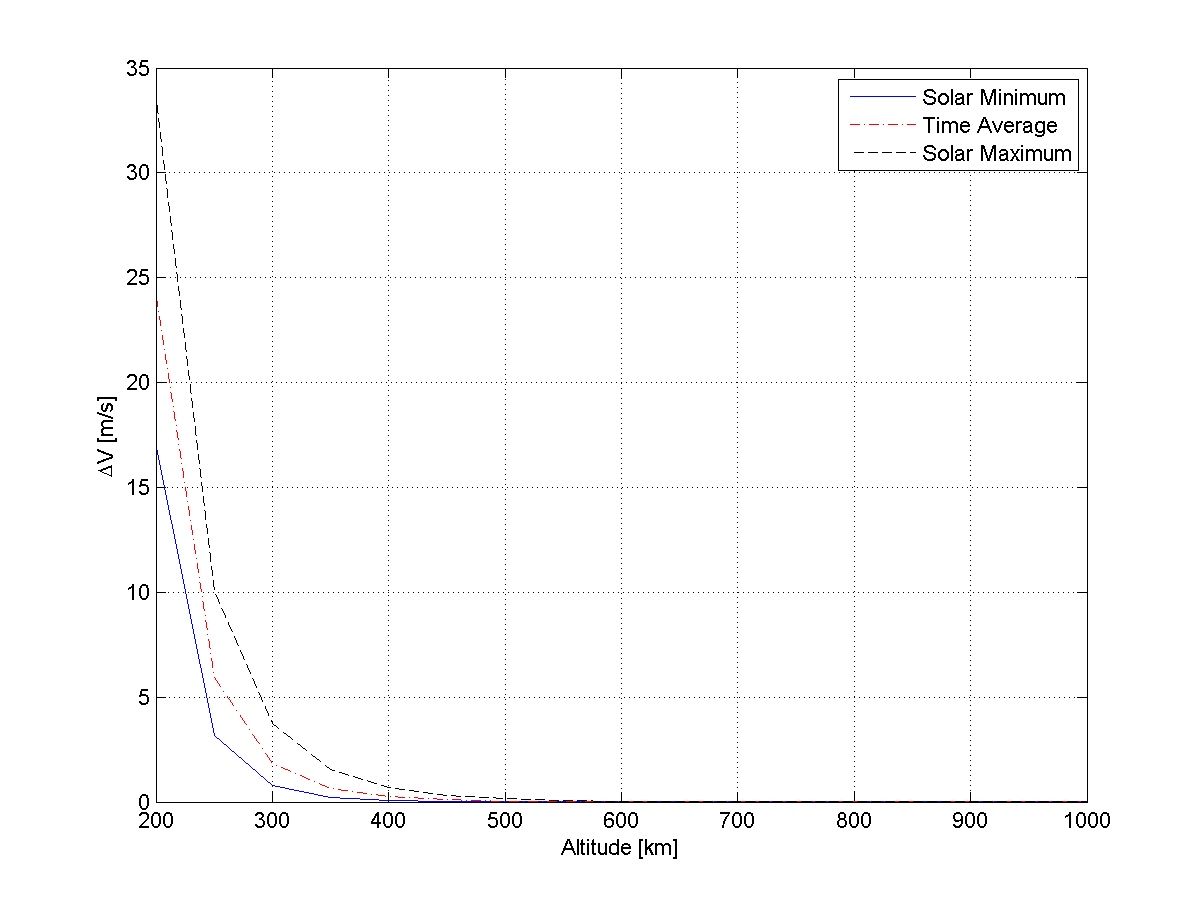
\includegraphics[width=0.95\textheight, angle=90]{chapters/img/deltaVEmitter.png}
\label{fig:deltaVGraph1}
\caption{Total $\Delta V$ for a satellite with $C_D$ = 4, A = 6.1 $m^2$ and m = 200 kg. Estimates for a range of orbit altitudes and different solar cycle stages. (CHECK MASS AND AREA).}
\end{figure}

\begin{figure}[h!]
\centering
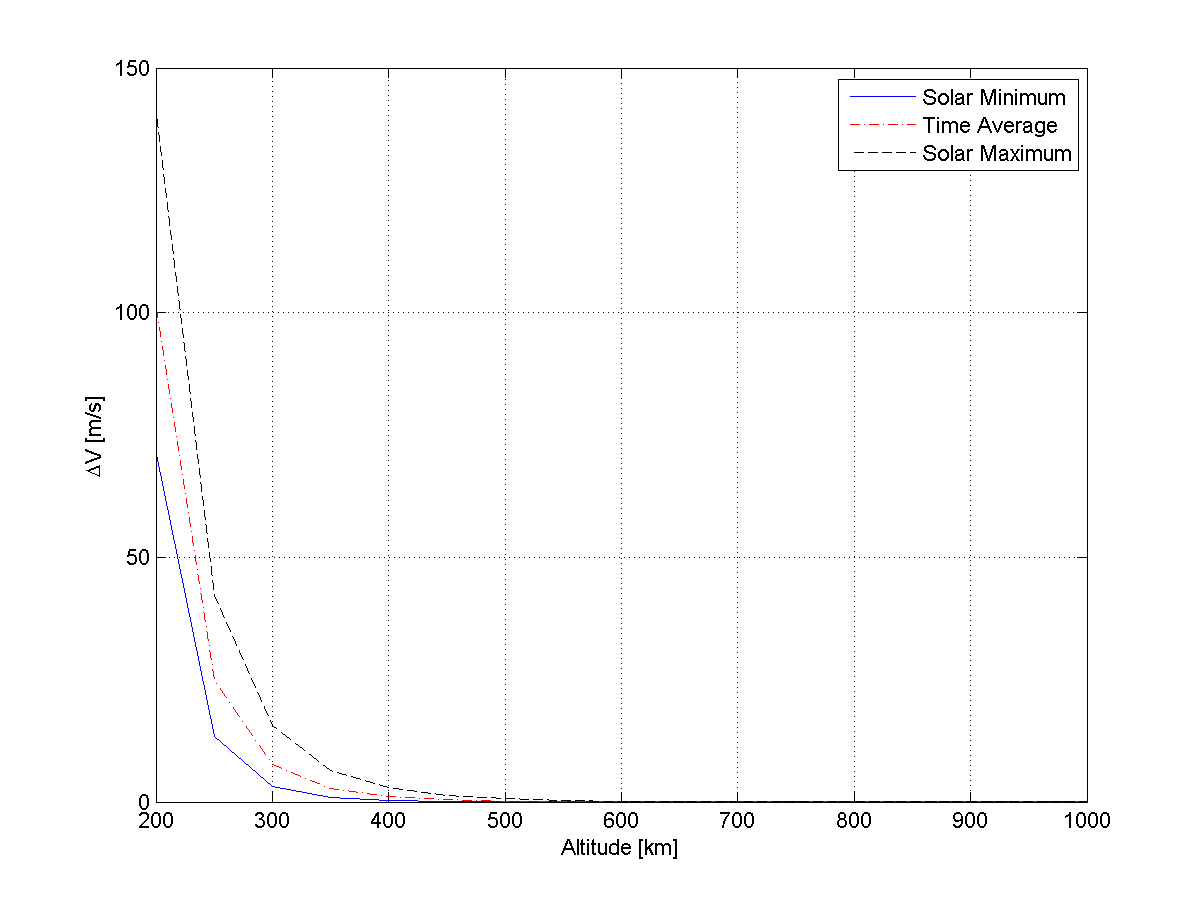
\includegraphics[width=0.95\textheight, angle=90]{chapters/img/deltaVReceiver.png}
\label{fig:deltaVGraph2}
\caption{Total $\Delta V$ for a satellite with $C_D$ = 4, A = 0.21 $m^2$ and m = 10 kg. Estimates for a range of orbit altitudes and different solar cycle stages. (CHECK MASS AND AREA).}
\end{figure}   

Three important conclusions can be drawn from the preceding analysis:
\begin{itemize}
	\item In order to avoid fast orbit degradation, and in turn greater mass due to propellant necessary to maintain orbit, the satellites should be placed as high as it is allowable by optical instruments. Based on drag analysis it is recommended to inject at 500 $\pm$ 25 km.
	\item The launch timeframe should be designed in such a way that the mission halftime falls under the solar minimum to reduce drag. This will also allow for a reduction in mass.
	\item The area/mass ratio for the emitter and receiver satellites should be designed as equivalent as possible. This will allow for slower constellation decay and for generally better stationkeeping.  
\end{itemize}
  

\subsection{Exposure to Particle Radiation}
\label{mtrRadiation}

In space, satellites are exposed to streams of highly energetic charged particles coming from the sun. Radiation from these particles can cause severe damage to satellite subsystems, including the payload. The main particle radiation source encountered by the swarm in the \ac{LEO} comes from the Van Allen Belts. These are regions around the Earth where charged particles (protons, electrons and ions) are trapped inside the magnetic field of the planet.

The total radiation dose consists of three components: proton dose, electron dose and the so-called Brehmsstrahlung X-Ray dose produced by the interaction between the electrons and the shielding material of the satellite. In \ac{LEO}, energetic protons in the inner radiation belt contribute most to the total radiation dose. This total is also strongly linked to the orbital altitude and below 1000 km will increase at approximately by the 5\textsuperscript{th} power of the altitude. Furthermore, just like with atmospheric drag, the solar activity plays a major role, thus all cases will be examined.

The number of particles trapped in the Van Allen belts in the vicinity of the orbit under question can be modeled using The Space Environment Information System (SPENVIS) that can be located at the following address: \emph{http://www.spenvis.oma.be/}. SPENVIS contains a large array of NASA and ESA (as well as other) tools and models for complex orbit analysis. For the purposes of this evaluation two models are used: AP-8 and AE-8. The first model predicts proton flux with energy levels above 100 MeV. The latter estimates the flux of electrons with energy of 0.5 MeV or above.

Figure \ref{fig:protFlux} on page \pageref{fig:protFlux} illustrates the trapped proton flux for solar minimum and maximum as a function of distance from Earth Center. It is evident that in \ac{LEO}, the proton flux stays relatively static w.r.t. solar activity. For the considered altitudes of 300 to 500 km (1.047 to 1.078 Earth radii) the satellites would encounter relatively the same order of magnitude of proton radiation. It is also evident that any higher altitude would mean a substantial increase in bombardment and hence reduction in the reliability of the subsystems.   

\begin{figure}
  \centering
  \subfloat[]{\label{fig:protMax}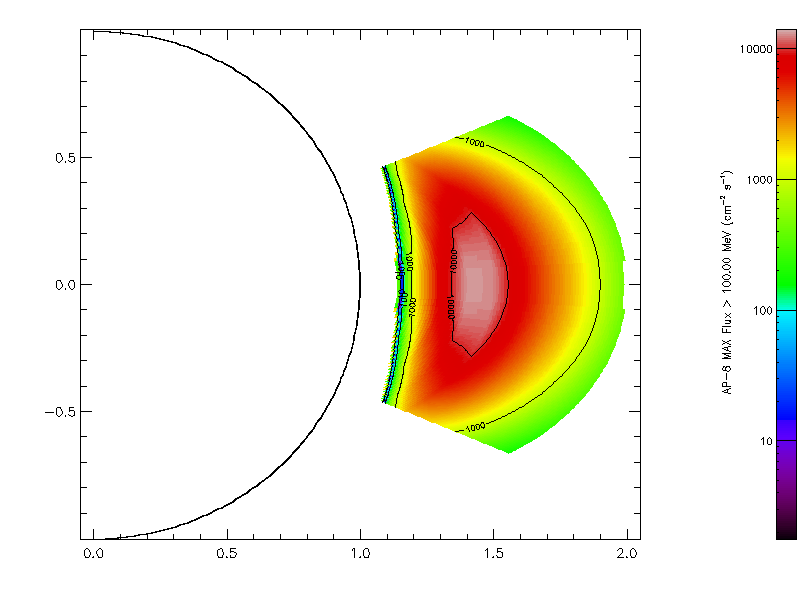
\includegraphics[width=0.7\textwidth]{chapters/img/protFluxMax.png}}\\                
  \subfloat[]{\label{fig:protMin}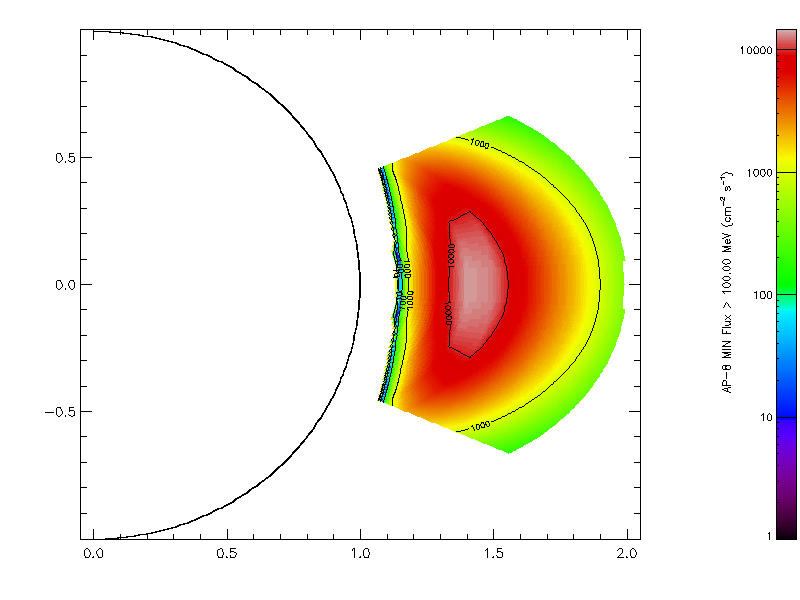
\includegraphics[width=0.7\textwidth]{chapters/img/protFluxMin.png}}
  \caption{AP-8 Proton Flux Model (energy $>$ 100 MeV) at solar maximum (a) and solar minimum (b) as a function of distance in mean Earth radii.}
  \label{fig:protFlux}
\end{figure}

Figure \ref{fig:elecFlux} on page \pageref{fig:elecFlux} illustrates the trapped electron flux for solar minimum and maximum as a function of distance from Earth Center. It is evident from this figure that lower altitudes would considerably reduce the radiation flux (up to one order of magnitude).

\begin{figure}
  \centering
  \subfloat[]{\label{fig:elecMax}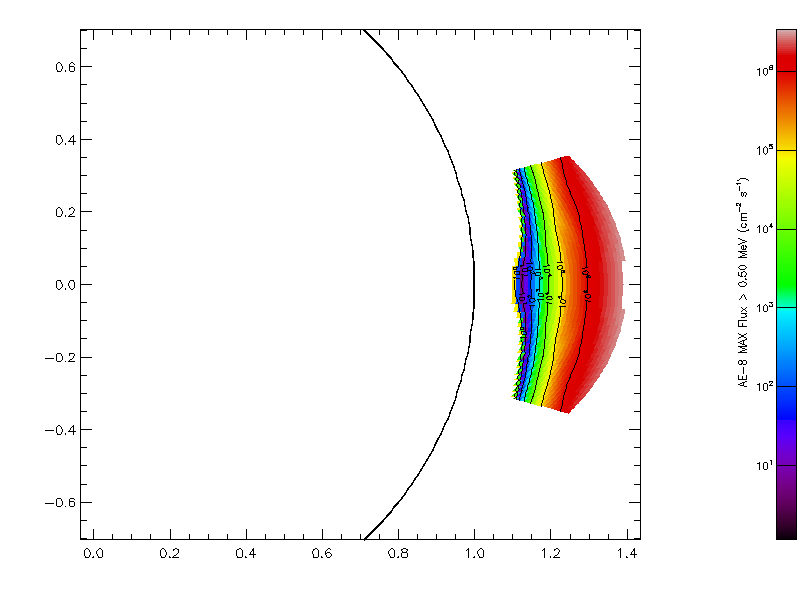
\includegraphics[width=0.7\textwidth]{chapters/img/elecFluxMax.png}}\\                
  \subfloat[]{\label{fig:elecMin}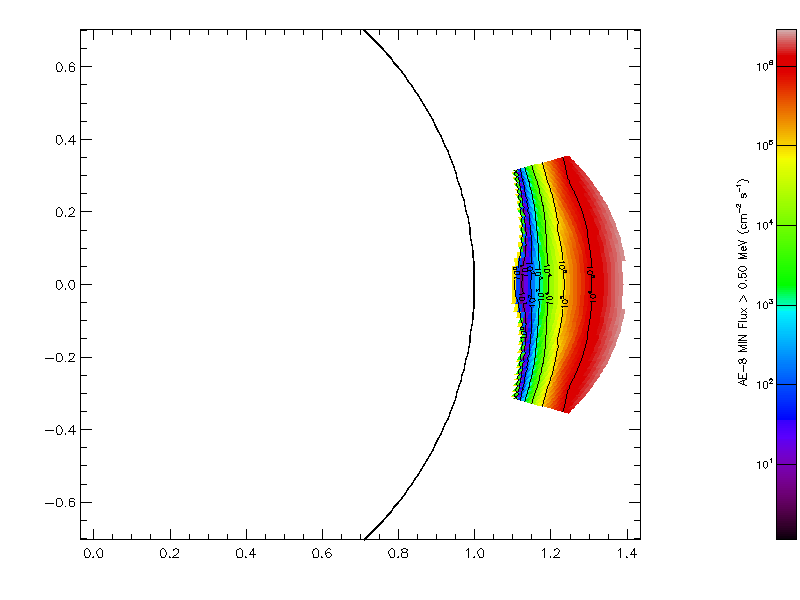
\includegraphics[width=0.7\textwidth]{chapters/img/elecFluxMin.png}}
  \caption{AE-8 Electron Flux Model (energy $>$ 0.5 MeV) at solar maximum (a) and solar minimum (b) as a function of distance in mean Earth radii.}
  \label{fig:elecFlux}
\end{figure}

Based on this data, the following conclusion emerges: while altitudes of around 500 km remain relatively safe, a lower orbit will result in a lower particle radiation flux, increasing reliability. Altitudes above 500 km become more and more dangerous for the mission.

\subsection{Conclusion}
\label{mtrAltConclusion}

ADD ALTITUDE CONCLUSION
